En el patio del colegio se ha pintado una zona de descanso con forma de cuadrado de lado 10 m. En el centro se dibuja una circunferencia que representa una zona decorativa donde no se puede transitar.

El resto del área del cuadrado corresponde a la zona disponible para los estudiantes.

\begin{center}
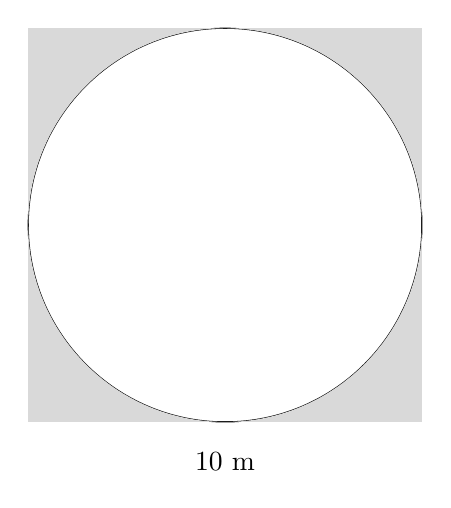
\begin{tikzpicture}[scale=0.5]

% Cuadrado
\draw (0,0) rectangle (10,10);

% Círculo inscrito
\draw (5,5) circle (5);

% Sombreado
\fill[gray!30, even odd rule]
(0,0) rectangle (10,10)
(5,5) circle (5);

\node at (5,-1) {10 m};

\end{tikzpicture}
\end{center}

Calcule el área disponible para los estudiantes.

Explique su procedimiento y justifique cada uno de los pasos realizados. No se aceptan respuestas sin justificación.